\begin{frame}{RepoJudgeBench in numbers}
\begin{columns}[T]
\begin{column}{0.48\textwidth}
\begin{itemize}
  \item \NProcessed{} post-2025 tasks processed in their Docker images
  \item \alert{\NPairs{} pairs} from \NInstances{} PRs in \NRepos{} repositories
  \item median gold patch: \NGoldMedianLines{} lines, \NGoldMedianFiles{} files, \NGoldMedianHunks{} hunks
  \item \NPairsJudged{} pairs judged (no leakage, prompt $\leq$ 6k tokens)
\end{itemize}
\end{column}
\begin{column}{0.5\textwidth}
\textbf{Tests catch only \TestCatchRate{} of injected defects}
\begin{itemize}
  \item authorisation guards: \CatchAuth{}
  \item error handling: \CatchSES{}
  \item races: \CatchRace{}
  \item resource leaks: \CatchRL{}
\end{itemize}
\end{column}
\end{columns}
\end{frame}

\begin{frame}{Judging protocol}
\begin{itemize}
  \item \CJB{} pairwise prompt, verdict \texttt{[[A>B]]} / \texttt{[[B>A]]}; issue as user prompt, two unified diffs as answers.
  \item Judges: \NJudges{} open models (1.5--4B, \texttt{llama.cpp}, CPU) + a thinking condition.
  \item Forced verdict prefix $\rightarrow$ logits of \texttt{A} vs \texttt{B}: greedy verdict and $p_A$.
  \item Both orders for every pair; 95\% bootstrap CIs (resampling PRs).
  \item Control: 45 \CJB{} pairs (code generation, repair, test generation).
\end{itemize}
\end{frame}

\begin{frame}{Result 1: accuracy in the two regimes}
\centering
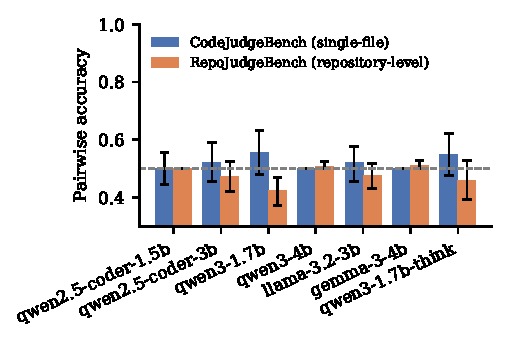
\includegraphics[width=0.62\textwidth]{../results/figures/regimes.pdf}

\small\SlideRegimeText{}
\end{frame}

\begin{frame}{Result 2: position bias and length bias}
\begin{itemize}
  \item \SlidePositionText{}
  \item After balanced position calibration, judges prefer the \alert{longer} patch in \PrefersLonger{} of unequal-length pairs.
  \item The defective variant is longer in \VarLongerShare{} of judged pairs, so judges systematically pick the defect.
  \item Benchmark artefact: a trivial ``pick the shorter patch'' rule scores \LengthHeurAcc{} --- future versions must length-match variants.
\end{itemize}
\end{frame}

\begin{frame}{Result 3: diff size and defect class}
\begin{columns}[T]
\begin{column}{0.5\textwidth}
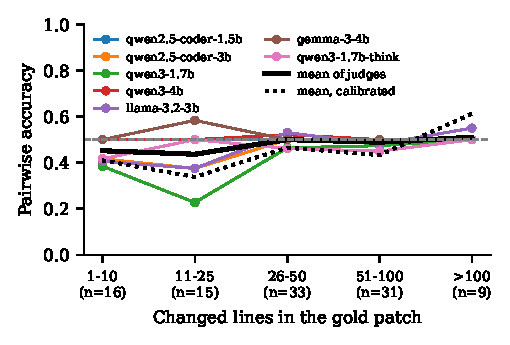
\includegraphics[width=\textwidth]{../results/figures/scaling.pdf}
\end{column}
\begin{column}{0.5\textwidth}
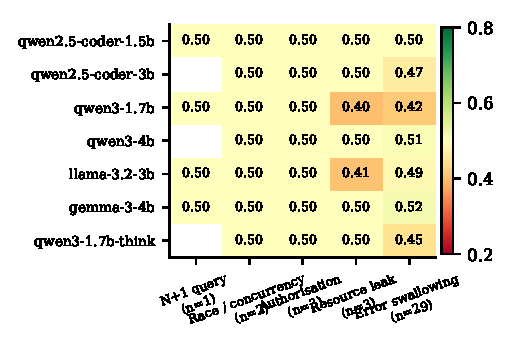
\includegraphics[width=\textwidth]{../results/figures/classes.pdf}
\end{column}
\end{columns}
\small\SlideScalingText{}
\end{frame}

\begin{frame}{Result 4: baselines and mitigation}
\begin{itemize}
  \item Static analysis with defect-targeted rules (Ruff/Bandit): \alert{\StaticRelAcc{}} --- flags the variant in \StaticRelFlagVar{} of pairs and never the gold patch.
  \item Static analysis with all rules: \StaticAllAcc{} (no signal).
  \item \SlideContextText{}
  \item \SlideThinkText{}
\end{itemize}
\end{frame}

\begin{frame}{Key findings}
\begin{enumerate}
  \item Tests miss most review-relevant defects: \TestCatchRate{} caught overall, resource leaks rarely.
  \item \SlideFindingTwo{}
  \item Verdicts are driven by \alert{position} and \alert{length}, not by the defect.
  \item Cheap targeted static analysis beats every small LLM judge on this task.
  \item Our benchmark itself has a length artefact --- a lesson for building judge benchmarks.
\end{enumerate}
\end{frame}
